\documentclass[tikz,border=10pt]{standalone}
\usepackage{amsmath}
\usepackage{amssymb}
\usetikzlibrary{calc, arrows.meta, decorations.pathreplacing}

\definecolor{vecorange}{HTML}{E65100} 
\definecolor{vecblue}{HTML}{1565C0}   
\definecolor{vecdark}{HTML}{BDBDBD}   
\definecolor{surfbg}{HTML}{9E9E9E}    
\definecolor{occluder}{HTML}{795548}  

\begin{document}
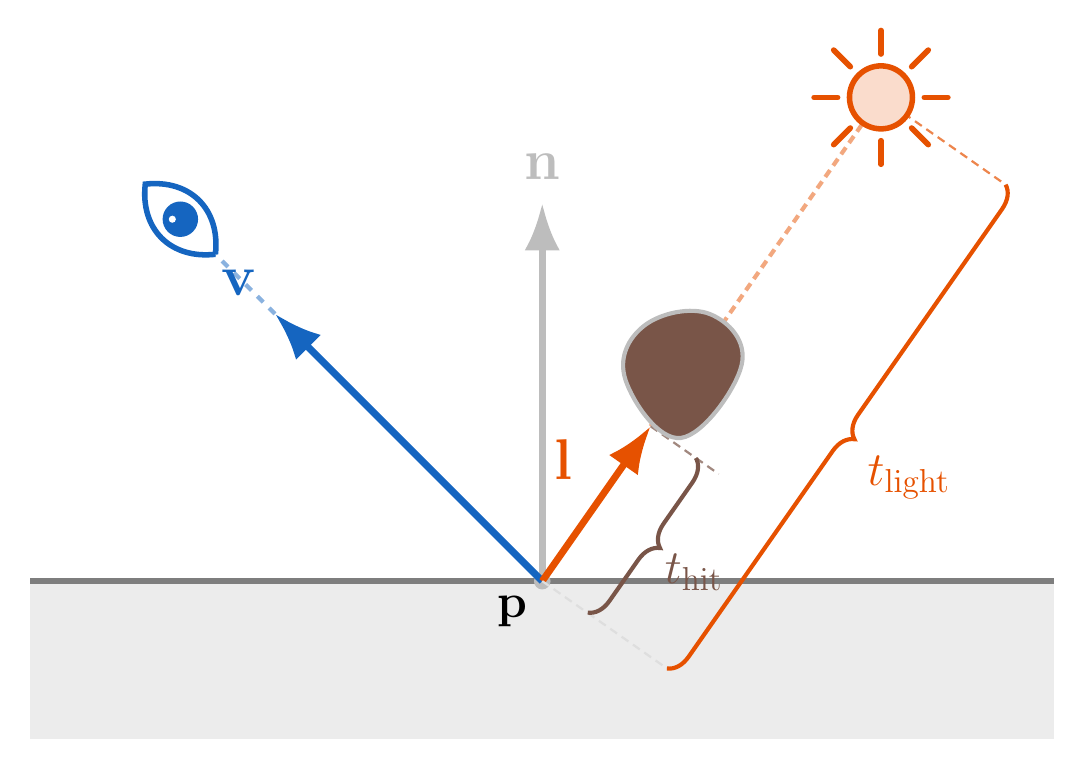
\begin{tikzpicture}[
    vec/.style={line width=2.5pt},
    >={Latex[length=6mm, width=4.5mm]}
]

\pgfmathsetmacro{\Vangle}{135}   
\pgfmathsetmacro{\Langle}{55}    
\pgfmathsetmacro{\vecLen}{4.8}
\pgfmathsetmacro{\SunDist}{7.5}
\pgfmathsetmacro{\EyeDist}{6.5}

% Surface (Deepened slightly to accommodate the new brace labels below)
\fill[surfbg!20] (-6.5, -2) rectangle (6.5, 0);
\draw[line width=2pt, surfbg!80!black] (-6.5, 0) -- (6.5, 0);

% Origin
\coordinate (O) at (0,0);
\fill[vecdark] (O) circle (3pt);
\node[below left=2pt, font=\LARGE] at (O) {$\mathbf{p}$};

% Normal
\draw[->, vec, vecdark] (O) -- (90:\vecLen) node[above=4pt, font=\huge] {$\mathbf{n}$};

% View Ray
\coordinate (Vtip) at (\Vangle:\vecLen);
\draw[->, vec, vecblue] (O) -- (Vtip) node[above left=2pt, font=\huge] {$\mathbf{v}$};

% Shadow Ray to Occluder (Label moved to above left to make room for braces)
\coordinate (OccluderPos) at (\Langle:3.2);
\draw[->, vec, vecorange] (O) -- (\Langle:2.4) node[midway, above left=4pt, font=\huge] {$\mathbf{l}$};

% Blocked Ray to Sun
\coordinate (SunPos) at (\Langle:\SunDist);
\draw[line width=1.5pt, vecorange, densely dashed, opacity=0.5] (\Langle:2.4) -- (SunPos);

% ---------------------------------------------------------
% BRACES FOR DISTANCES (t_hit and t_light)
% ---------------------------------------------------------

% Subtle dashed projection lines to bracket the distances clearly
\draw[vecdark!50, thick, densely dashed] (O) -- ++(\Langle-90:55pt);
\draw[occluder!70, thick, densely dashed] (\Langle:2.4) -- ++(\Langle-90:30pt);
\draw[vecorange!70, thick, densely dashed] (SunPos) -- ++(\Langle-90:55pt);

% t_hit Brace (Drawing from Occluder to Origin places it on the bottom-right)
\draw[decorate, decoration={brace, amplitude=8pt, raise=20pt}, line width=1.5pt, occluder]
    (\Langle:2.4) -- (O) node[midway, shift={(\Langle-90:43pt)}, font=\LARGE, text=occluder] {$t_{\text{hit}}$};
    
% t_light Brace
\draw[decorate, decoration={brace, amplitude=8pt, raise=55pt}, line width=1.5pt, vecorange]
    (SunPos) -- (O) node[midway, shift={(\Langle-90:87pt)}, font=\LARGE, text=vecorange] {$t_{\text{light}}$};

% ---------------------------------------------------------

% Occluder
\begin{scope}[shift={(OccluderPos)}, rotate=\Langle]
    \draw[fill=occluder, draw=vecdark, line width=1.5pt] plot[smooth cycle, tension=0.7] coordinates {
        (-0.7, -0.4) (0.5, -0.5) (0.8, 0.2) (0.2, 0.8) (-0.5, 0.6)
    };
\end{scope}

% Viewer (Eye) Context
\coordinate (EyePos) at (\Vangle:\EyeDist);
\draw[line width=1.5pt, vecblue, dashed, opacity=0.5] (Vtip) -- (EyePos);
\begin{scope}[shift={(EyePos)}, rotate=\Vangle, scale=0.9]
    \fill[white] (0,0) ellipse (0.7 and 0.4);
    \draw[line width=2pt, vecblue] (-0.7,0) .. controls (-0.3,0.5) and (0.3,0.5) .. (0.7,0)
                            .. controls (0.3,-0.5) and (-0.3,-0.5) .. (-0.7,0);
    \fill[vecblue] (0,0) circle (0.25);
    \fill[white] (0.08,0.08) circle (0.05); 
\end{scope}

% Light Source (Sun) Context
\begin{scope}[shift={(SunPos)}]
    \fill[vecorange!20] (0,0) circle (0.4);
    \draw[vecorange, line width=2pt] (0,0) circle (0.4);
    \foreach \a in {0, 45, ..., 315} {
        \draw[vecorange, line width=2pt, line cap=round] (\a:0.55) -- (\a:0.85);
    }
\end{scope}

\end{tikzpicture}
\end{document}